%% ===================================================================
%%  CSE 402: Numerical Analysis, Simulation and Modeling Sessional
%%  Final report, ACM "acmart" sigconf template.
%%
%%  BUILD:   build.bat          (Windows)
%%           make               (make / latexmk)
%%           or manually:
%%           pdflatex main -> bibtex main -> pdflatex main -> pdflatex main
%%
%%  >>> EDIT THESE TWO LINES BEFORE SUBMITTING <<<
%% ===================================================================
\newcommand{\GROUPNUM}{02}                                  % <-- your group number
\newcommand{\REPOURL}{https://github.com/Ahnaf-Akib-Tanim/Numeric-Project-submission}  % <-- your public repo
%% ===================================================================

\documentclass[sigconf,nonacm]{acmart}

\usepackage{booktabs}
\usepackage{multirow}
\usepackage{amsmath}
% NB: do not load amssymb. It clashes with acmart's newtx math setup
% ("Command \Bbbk already defined") and nothing here needs it.
\usepackage{graphicx}
\usepackage{algorithm}
\usepackage{algpseudocode}
\usepackage{xcolor}

% --- course report, not a real ACM submission --------------------------
\settopmatter{printacmref=false}
\renewcommand\footnotetextcopyrightpermission[1]{}
\pagestyle{plain}
\setcopyright{none}

\definecolor{hl}{HTML}{184F95}
\newcommand{\best}[1]{\textbf{#1}}

\begin{document}

\title{Discrete-Event Simulation and Constrained Optimisation of
       Emergency-Department Patient Flow}
% acmart's \subtitle takes plain text only, so no line breaks or math.
\subtitle{A From-Scratch Replication of Lv et al. (2026) and Four Extensions}
\titlenote{CSE 402: Numerical Analysis, Simulation and Modeling Sessional.
           \textbf{Group \GROUPNUM, Section C.} Code and all generated results:
           \url{\REPOURL}}

\author{Sudip Kumar Saha}
\affiliation{%
  \institution{Student ID 2105152}
  \city{CSE}
  \country{BUET}}
\email{2105152@ugrad.cse.buet.ac.bd}

\author{Ahnaf Akib Tanim}
\affiliation{%
  \institution{Student ID 2105154}
  \city{CSE}
  \country{BUET}}
\email{2105154@ugrad.cse.buet.ac.bd}

\author{Md. Shahjalal Rumman}
\affiliation{%
  \institution{Student ID 2105165}
  \city{CSE}
  \country{BUET}}
\email{2105165@ugrad.cse.buet.ac.bd}

\author{Md. Dulal Hossain}
\affiliation{%
  \institution{Student ID 2105169}
  \city{CSE}
  \country{BUET}}
\email{2105169@ugrad.cse.buet.ac.bd}

\author{Md. Shoaib Hossain}
\affiliation{%
  \institution{Student ID 2105170}
  \city{CSE}
  \country{BUET}}
\email{2105170@ugrad.cse.buet.ac.bd}

\renewcommand{\shortauthors}{Saha, Tanim, Rumman, Hossain and Hossain,
                             Group \GROUPNUM, Section C}

%% ======================================================================
\begin{abstract}
Every time a physician in an emergency department (ED) becomes free, someone
has to decide which of three queues to serve next: newly arrived urgent
patients, newly arrived non-urgent patients, or patients coming back for a
follow-up after their diagnostics. Lv et al.\ (2026) studied this problem with
a discrete-event simulation (DES) of a Chinese tertiary-hospital ED and
compared three physician-scheduling heuristics. We rebuilt that simulation from
scratch, checked it against every KPI the paper publishes, and then extended it
in four ways. First, we added the c$\mu$ rule and its generalisation, two
scheduling policies that come with optimality results for a stated delay-cost
objective instead of being designed by hand. Second, we replaced the paper's
two-stage grid search over the slack thresholds $(k_1,k_2)$ with our own
Nelder--Mead implementation, using a sample-average approximation and an
exterior penalty for the service-level constraint. Third, we built a weekly
cost model and used it to optimise the integer physician roster together with
the thresholds. Fourth, we used exact common random numbers (CRN) and measured
how much variance they remove. Our rebuild reproduces all six structural
findings of the paper, and its equipment-utilisation figures agree with the
published table to within $0.5$ percentage points. Absolute waiting times come
out $12$--$25\%$ higher, which we attribute to the high implied load
$\rho\approx0.87$. Nelder--Mead gets within $0.006$ minutes of the grid-search
optimum while using $19\times$ fewer simulations, the cost-optimal roster lowers
weekly cost by $20.7\%$, and CRN removes $98.9\%$ of the variance in policy
comparisons. We also found that the thresholds published in the paper do not
satisfy the service-level constraint on our model, so they need to be re-tuned
rather than reused.
\end{abstract}

\begin{CCSXML}
<ccs2012>
<concept>
<concept_id>10010405.10010481.10010487</concept_id>
<concept_desc>Applied computing~Health informatics</concept_desc>
<concept_significance>500</concept_significance>
</concept>
<concept>
<concept_id>10003752.10010070.10010071.10010261</concept_id>
<concept_desc>Theory of computation~Scheduling algorithms</concept_desc>
<concept_significance>500</concept_significance>
</concept>
<concept>
<concept_id>10010147.10010341.10010342.10010343</concept_id>
<concept_desc>Computing methodologies~Discrete-event simulation</concept_desc>
<concept_significance>500</concept_significance>
</concept>
<concept>
<concept_id>10002950.10003705.10011686</concept_id>
<concept_desc>Mathematics of computing~Nonconvex optimization</concept_desc>
<concept_significance>300</concept_significance>
</concept>
</ccs2012>
\end{CCSXML}

\ccsdesc[500]{Applied computing~Health informatics}
\ccsdesc[500]{Computing methodologies~Discrete-event simulation}
\ccsdesc[500]{Theory of computation~Scheduling algorithms}
\ccsdesc[300]{Mathematics of computing~Nonconvex optimization}

\keywords{discrete-event simulation, emergency department, patient scheduling,
          c$\mu$ rule, Nelder--Mead, simulation optimisation, common random
          numbers, variance reduction, staffing}

\maketitle

%% ======================================================================
\section{Introduction and Base Paper Review}

\subsection{Background}
Emergency departments are one of the main congestion points in a hospital.
Demand is random and changes a lot over the day and the week, service times
vary from patient to patient, and the key resource, physician time, is limited
and expensive. Patients are triaged into urgency levels that each have their
own waiting target, so an ED can be modelled as a multi-class queue with
deadlines. Simulation is the usual way to evaluate operating policies in this
setting~\cite{vanbrabant2019kpi,wang2023simopt}, since time-varying arrivals,
non-exponential service and history-dependent priority rules make exact
analysis impractical~\cite{huang2015control}.

\subsection{The base paper}
Our base paper is Lv, Liu, Yan and Wang~\cite{lv2026des}. It builds a DES of a
Grade-A tertiary-hospital ED in China and limits it to triage Level~III
(urgent) and Level~IV (non-urgent) patients, who make up most ED visits.
Patients arrive according to a non-homogeneous Poisson process whose rate
$\lambda_{d,h}$ depends on the day and hour. Each patient waits for an
\emph{initial} consultation and may then need diagnostics (laboratory, X-ray,
CT or B-ultrasound). Patients who do need diagnostics come back afterwards and
compete for the same physicians in a \emph{follow-up} queue. Physicians work
three shifts per day, staffed $(5,5,3)$.

The paper compares three physician-scheduling policies within one simulation
framework:

\begin{itemize}
\item \textbf{Initial-First (IFP)}: new arrivals always come first, Level III
      before Level IV, and follow-ups are served only when there is capacity
      left over.
\item \textbf{Alternating 1:1 (ALT)}: at most half the physicians may do
      initial consultations at any time, and the rest take follow-ups.
\item \textbf{Slack-Based (SBP)}: a patient of level $\ell$ is flagged
      \emph{urgent} once their waiting time reaches $T_\ell - k_\ell$, where
      $T_\ell$ is the triage target and $k_\ell$ is a tunable slack
      parameter~\cite{davenport2001slack}. The priority order is then
      urgent-L3 $>$ urgent-L4 $>$ follow-up $>$ non-urgent initial.
\end{itemize}

The SBP thresholds are tuned by a two-stage grid search (coarse step $1.0$,
then fine step $0.1$). The paper reports an optimum of $(k_1,k_2)=(13.1,2.1)$
and a drop in mean waiting time from $46.26$~min under IFP to $35.25$~min, a
$23.8\%$ reduction, with no service-level violations. Significance is tested
with paired $t$-tests, a Bonferroni correction and Cohen's $d$.

\subsection{Gaps and objectives}
The base paper is a careful comparison, but there are several things it does
not do, listed in Table~\ref{tab:gaps}. Its source code and operational dataset
are also not public. Only summary statistics are published, but these turned
out to be enough to rebuild an equivalent simulator.

\begin{table}[t]
\caption{Gaps in the base paper and the corresponding contribution of this work.}
\label{tab:gaps}
\small
\begin{tabular}{@{}p{2.9cm}p{2.9cm}p{1.6cm}@{}}
\toprule
\textbf{Paper does} & \textbf{Paper does not} & \textbf{Our work} \\
\midrule
Grid-search two thresholds & Optimise the \emph{staffing level} jointly & \S\ref{sec:cost} \\
Compare three heuristics & Compare against a provably optimal rule & \S\ref{sec:cmu} \\
Brute-force search & Use a derivative-free numerical optimiser & \S\ref{sec:opt} \\
100 independent replications & Apply variance reduction & \S\ref{sec:crn} \\
Report results & Release engine or data & \S\ref{sec:impl} \\
\bottomrule
\end{tabular}
\end{table}

Our objectives were therefore to: (i)~rebuild the model from scratch and see
how closely the published results can be reproduced from the published
parameters alone; (ii)~add a scheduling rule that comes from queueing theory
instead of being designed by hand; (iii)~replace the grid search with a proper
numerical optimiser under an explicit constraint, and measure the saving in a
way that does not depend on hardware; (iv)~answer the staffing question that
the paper only looks at through sensitivity analysis; and (v)~make the
statistical comparison sharper through variance reduction.

%% ======================================================================
\section{Methodology}

\subsection{System model}
Let $t$ be simulated time in minutes over a horizon of one week
($T=10{,}080$). As in the paper, the day and hour indices are
\begin{equation}
d = \left\lfloor \tfrac{t}{1440} \right\rfloor \bmod 7,
\qquad
h = \left\lfloor \tfrac{t \bmod 1440}{60} \right\rfloor ,
\end{equation}
so the arrival rate $\lambda_{d,h}$ is piecewise constant and repeats every
week. Each arrival gets triage level $\ell\in\{3,4\}$ with probabilities $0.25$
and $0.75$, and the matching waiting target $T_3=30$ or $T_4=120$ minutes. The
state consists of three FIFO queues, $W^t_{\text{init},3}$,
$W^t_{\text{init},4}$ and $W^t_{\text{follow}}$, which share $R^t$ physicians.

\subsection{Discrete-event engine}
The simulator is our own event loop built on a binary min-heap. We did not use
a process-oriented simulation library, so every mechanism the paper describes
appears explicitly in the code. Each event is a 4-tuple
$(\textit{time},\textit{type},\textit{seq},\textit{payload})$ ordered
lexicographically. The increasing counter \textit{seq} breaks ties, which makes
the ordering total and each replication exactly reproducible. There are five
event types: shift change, arrival, consultation end, examination device
release and examination results ready. After each event the engine calls a
single \textsc{Dispatch} routine, and this is the only place where the
scheduling policy is applied (Algorithm~\ref{alg:loop}). Changing the policy
therefore touches no other part of the simulator, so all policies run under
the same mechanics.

\begin{algorithm}[t]
\caption{Discrete-event main loop}
\label{alg:loop}
\begin{algorithmic}[1]
\State push all arrivals and shift changes onto the heap $H$
\While{$H \neq \emptyset$}
  \State $e \gets \textsc{PopMin}(H)$
  \If{$e.\textit{time} \ge T$} \textbf{break} \EndIf
  \State $\textit{now} \gets e.\textit{time}$; accrue utilisation integrals
  \State apply the state transition of $e$
  \State $R \gets \textsc{FreePhysicians}(\textit{now})$
  \If{$R>0$ and some queue is non-empty}
    \State $P \gets \textsc{Policy.Allocate}(\textit{state},\textit{now},R)$
    \State start service for every patient in $P$
  \EndIf
\EndWhile
\end{algorithmic}
\end{algorithm}

Service is non-preemptive. When staffing drops at 22:00, consultations already
in progress continue, and no new consultation starts until the number of busy
physicians falls below the new capacity.

\subsection{Arrival generation by thinning}
Since $\lambda(t)$ is a step function with 168 pieces, inverting its cumulative
intensity is easy to get wrong. We sample the process by Lewis--Shedler
thinning~\cite{lewis1979thinning} instead. With
$\lambda^{*}=\max_{d,h}\lambda_{d,h}=23.05$/h, we generate a homogeneous
process of rate $\lambda^{*}$ by adding up $\mathrm{Exp}(1/\lambda^{*})$ gaps,
and keep each candidate time $t$ with probability $\lambda(t)/\lambda^{*}$. In
a small interval $\mathrm{d}t$ a candidate appears with probability
$\lambda^{*}\,\mathrm{d}t$ and is kept with probability
$\lambda(t)/\lambda^{*}$, so the kept points have intensity $\lambda(t)$
exactly. About $58\%$ of candidates are accepted.

\subsection{Service times by inverse-CDF sampling}
Consultation times follow truncated exponentials $\mathrm{TruncExp}(\lambda_k,
[a_k,b_k])$. Inverting the truncated CDF gives
\begin{equation}
x = -\frac{1}{\lambda}
    \ln\!\left( e^{-\lambda a} - u\,(e^{-\lambda a}-e^{-\lambda b}) \right),
\qquad u\sim U(0,1),
\label{eq:truncexp}
\end{equation}
which uses exactly one uniform per variate. We chose this on purpose.
Rejection sampling uses a variable number of uniforms, which would break the
stream synchronisation that \S\ref{sec:crn} relies on. The mean after
truncation has a closed form,
\begin{equation}
\mathbb{E}[X] = a + \frac{1}{\lambda}
  - \frac{(b-a)\,e^{-\lambda(b-a)}}{1-e^{-\lambda(b-a)}} ,
\label{eq:truncmean}
\end{equation}
which gives $9.093$~min for initial and $12.841$~min for follow-up
consultations. One detail of the paper needs comment here. A truncated
exponential on $[5,25]$ cannot have a mean of $15$~min, because $15$ is only
the limit as $\lambda\to0$ and is never reached. So $\lambda_2=1/15$ is the
only reading that fits the paper's stated bounds, and it is also the reading
that reproduces the reported physician utilisation of about $85\%$.

\subsection{Scheduling policies}
\label{sec:cmu}
We implement IFP, ALT and SBP directly from Equations (8)--(23) of the base
paper, and add two policies taken from queueing theory.

\paragraph{The c$\mu$ rule (WSEPT).}
Cox and Smith~\cite{cox1961queues}, with a later proof by Buyukkoc et
al.~\cite{buyukkoc1985cmu}, showed that for a multi-class queue served by a
single pool with \emph{linear} holding costs $c_\ell$ per unit of waiting,
expected total holding cost is minimised by always serving the non-empty class
with the largest index
\begin{equation}
I_\ell = c_\ell\,\mu_\ell ,
\qquad \mu_\ell = 1/\mathbb{E}[S_\ell] .
\label{eq:cmu}
\end{equation}
We set $c_\ell = 1/T_\ell$, so a minute of waiting costs more for classes that
can tolerate less waiting. This turns the triage targets directly into delay
costs. Table~\ref{tab:cmu} lists the resulting indices. The rule is also known
as Weighted Shortest Expected Processing Time (WSEPT). Because its indices are
constants, it reduces to a fixed priority order (L3 initial $>$ follow-up $>$
L4 initial). This follows from the theorem itself, and it is the limitation
that the generalised rule addresses.

\paragraph{The generalised c$\mu$ rule (Gc$\mu$).}
For \emph{convex} delay costs $C_\ell(w)$, Van Mieghem~\cite{vanmieghem1995gcmu}
and Mandelbaum and Stolyar~\cite{mandelbaum2004convex} show that the
asymptotically optimal index is $C_\ell'(w)\,\mu_\ell$, evaluated at the
head-of-line delay. With $C_\ell(w)=(w/T_\ell)^2$ this becomes
\begin{equation}
I_\ell(t) = \frac{2\,w_{\text{head}}\,\mu_\ell}{T_\ell^{2}} ,
\label{eq:gcmu}
\end{equation}
so the index increases with how long the patient at the front of the queue has
been waiting. Like SBP, Gc$\mu$ reacts to waiting time, but it follows from the
cost function rather than from tuning, and it has no free parameters.

\begin{table}[t]
\caption{Index values computed by the c$\mu$ and generalised c$\mu$ rules under
         the base paper's parameters.}
\label{tab:cmu}
\small
\begin{tabular}{@{}lrrrr@{}}
\toprule
\textbf{Class} & $T_\ell$ & $\mathbb{E}[S_\ell]$ & $c_\ell$ & $\mathbf{c_\ell\mu_\ell}$ \\
\midrule
Level III initial & 30  & 9.093  & 0.03333 & \best{0.003666} \\
Follow-up         & 60  & 12.841 & 0.01667 & \best{0.001298} \\
Level IV initial  & 120 & 9.093  & 0.00833 & \best{0.000916} \\
\bottomrule
\end{tabular}
\end{table}

\paragraph{A fair objective.}
The c$\mu$ rule is optimal for holding cost, not for the unweighted mean wait,
so it would be unfair to judge it on the mean wait alone. We therefore also
report the \emph{holding cost}
\begin{equation}
H = \frac{1}{N}\sum_{i=1}^{N} \frac{w_i}{T_{\ell(i)}} ,
\label{eq:holding}
\end{equation}
which measures each patient's wait relative to their own clinical target.

\subsection{Constrained simulation optimisation}
\label{sec:opt}
The tuning problem in the base paper is
\begin{equation}
\min_{k_1,k_2}\ \overline{W}_{\text{total}}(k_1,k_2)
\quad \text{s.t.} \quad SL_\ell(k_1,k_2) \ge SL^{\min}_\ell,\ \ell\in\{3,4\}.
\label{eq:problem}
\end{equation}
We needed three changes to make it suitable for a simplex method.

\paragraph{Sample average approximation.}
Simulation outputs are noisy, and simplex methods tend to stall on noisy
surfaces. We therefore minimise the average over a \emph{fixed} set of $n$
patient streams~\cite{kim2015saa}. Since the engine is deterministic for a given
stream, $\hat{F}$ is a deterministic function, and evaluating the same point
twice gives the same value. Using the same streams for every candidate also
cancels much of the noise between points, so the surface is far smoother than
the noise of a single run would suggest.

\paragraph{Exterior penalty.}
Nelder--Mead only handles unconstrained problems, so we add the service-level
constraint as a penalty:
\begin{equation}
F(k_1,k_2) = \overline{W}_{\text{total}}
 + \mu \sum_{\ell\in\{3,4\}} \max\!\left(0,\ SL^{\min}_\ell - SL_\ell\right),
\label{eq:penalty}
\end{equation}
with $\mu = 500$ minutes per unit of shortfall. In other words, missing the
service level by one percentage point costs the same as five extra minutes of
average waiting~\cite{nocedal2006numerical}. This is large enough that an
infeasible point never comes out as the optimum, but small enough that the
penalised surface stays smooth near the boundary. The bounds $k\ge0$ are
enforced by \emph{projection}, which lets the simplex move along a bound
instead of being pushed away from it.

\paragraph{Nelder--Mead.}
We wrote the downhill simplex method~\cite{nelder1965simplex} ourselves
(Algorithm~\ref{alg:nm}) with the standard coefficients $\alpha=1$, $\gamma=2$,
$\rho=0.5$, $\sigma=0.5$. Two details mattered in practice. First, the initial
simplex uses a separate step for each dimension, $(4,15)$, because $k_1$ ranges
over roughly $[0,30]$ (against $T_3=30$) while $k_2$ ranges over roughly
$[0,120]$ (against $T_4=120$). A single step size would give a poorly
conditioned simplex. Second, since the method is local, we run it from four
different starting points and report how much the results differ.

\begin{algorithm}[t]
\caption{Nelder--Mead iteration (minimisation)}
\label{alg:nm}
\begin{algorithmic}[1]
\State order vertices so that $f(x_1)\le\cdots\le f(x_{n+1})$
\State \textbf{stop} if simplex span $\le x_{\text{tol}}$ and
       $f(x_{n+1})-f(x_1)\le f_{\text{tol}}$
\State $x_c \gets \frac{1}{n}\sum_{i\le n} x_i$ \Comment{centroid without worst}
\State $x_r \gets \Pi\!\left(x_c + \alpha (x_c - x_{n+1})\right)$ \Comment{reflect}
\If{$f(x_r) < f(x_1)$}
  \State $x_e \gets \Pi\!\left(x_c + \gamma (x_r - x_c)\right)$ \Comment{expand}
  \State $x_{n+1} \gets \arg\min\{f(x_e),f(x_r)\}$
\ElsIf{$f(x_r) < f(x_n)$}
  \State $x_{n+1} \gets x_r$
\Else
  \State $x_k \gets \Pi\!\left(x_c + \rho\,(\cdot - x_c)\right)$ \Comment{contract}
  \If{improved} $x_{n+1} \gets x_k$
  \Else\ $x_i \gets \Pi\!\left(x_1 + \sigma (x_i - x_1)\right)\ \forall i>1$
  \EndIf
\EndIf
\end{algorithmic}
\end{algorithm}

Here $\Pi(\cdot)$ is projection onto the box. We measure the optimiser's cost
in \emph{week-long simulations} rather than seconds, so the comparison with the
paper's grid does not depend on hardware or on how many processes run in
parallel.

\subsection{Cost-based staffing}
\label{sec:cost}
The paper varies staffing levels but cannot recommend one, because it has no
way to compare the cost of a physician-hour with the cost of a minute of
patient waiting. We add that missing objective:
\begin{equation}
C(R,k_1,k_2) = \alpha H_{\text{phys}} + \beta W_{\text{total}}
             + \gamma V_{\text{SLA}} ,
\label{eq:cost}
\end{equation}
where $R=(R_{\text{m}},R_{\text{a}},R_{\text{n}})$ is the integer roster,
$H_{\text{phys}}$ is rostered physician-hours per week, $W_{\text{total}}$ is
total patient waiting-minutes per week and $V_{\text{SLA}}$ is the number of
patients who waited past their triage target. Good thresholds for a night
shift with 3 physicians are not the same as good thresholds for one with 5, so
we re-optimise $(k_1,k_2)$ inside each candidate roster. Roster and thresholds
are therefore optimised together rather than one after the other. The search
has two stages. First, we screen every roster in $\{2,\dots,8\}^3$, except those
with more physicians at night than during the day, and drop the unstable ones.
A roster counts as unstable if more than $15\%$ of the week's patients are
still in the system at the end of the horizon, which means the queue is
growing instead of clearing. The best remaining candidates then get a full
Nelder--Mead re-tune.

\subsection{Common random numbers and inference}
\label{sec:crn}
For two policies $A$ and $B$,
\begin{equation}
\operatorname{Var}(A-B) = \operatorname{Var}(A) + \operatorname{Var}(B)
                        - 2\operatorname{Cov}(A,B).
\label{eq:crn}
\end{equation}
With independent streams the covariance is zero. Under CRN both policies see
the same simulated week, so a busy week raises both results together. The
covariance becomes strongly positive and the variance of the
\emph{difference} drops sharply, while each policy's own variance stays the
same~\cite{law2015simulation}.

In practice much of this benefit is often lost through desynchronisation: once
two policies start making different decisions, they use random numbers in a
different order. We prevent this by design. From one seed we spawn six
independent PCG64 substreams~\cite{oneill2014pcg} (arrivals, triage levels,
initial service, follow-up service, examination need, examination selection).
The whole exogenous patient stream, including arrival times, levels, both
consultation durations and required diagnostics, is generated \emph{before}
the run starts, so the engine draws no random numbers during the simulation.
Each variate also uses exactly one uniform, by Eq.~\eqref{eq:truncexp}. As a
result, patient $\#1723$ (or any other) is identical under every policy.

For inference we follow the base paper: paired $t$-tests on the
per-replication means (paired because CRN makes the design paired), a
Bonferroni correction across the family of comparisons, and Cohen's $d$ in its
paired form $\bar{d}/s_d$. We also report the smallest $n$ that satisfies
$t_{0.975,n-1}\,s/\sqrt{n} \le h$, found by iteration because the $t$ quantile
itself depends on $n$.

%% ======================================================================
\section{Implementation and Experiments}
\label{sec:impl}

\subsection{Software}
The simulator is written in Python 3.11 and has about $7{,}900$ lines in
total: a $15$-module library, $10$ experiment scripts and a verification suite
with $33$ checks. We use only NumPy~\cite{harris2020numpy},
SciPy~\cite{virtanen2020scipy}, Matplotlib~\cite{hunter2007matplotlib} and
pandas. SciPy is used only for distribution quantiles, the $t$-distribution,
and as an independent check on our own optimiser. The library follows the
five-module structure of the base paper's Figure~2 (entity definition, event
scheduling, resource scheduling, strategy execution and statistical output),
so the code and the paper can be read side by side. All code is available at
\url{\REPOURL}.

One implementation detail made a large difference. We first stored events as
an ordered dataclass, and profiling showed that Python-level comparisons inside
the heap took $22\%$ of the runtime. Switching to plain tuples moved these
comparisons into C and reduced the time per replication from $0.20$\,s to
$0.076$\,s. Without this change, the $50{,}415$-simulation grid search in
\S\ref{sec:resopt} would not have been practical.

\subsection{Parameters}
All parameters come from the base paper and are listed in
Table~\ref{tab:params}. The arrival rates are copied directly from its Table~2
($7\times24$ values). The offered load implied by these parameters is
\begin{equation}
\rho = \frac{N\left(\mathbb{E}[S_1] + p_{\text{exam}}\mathbb{E}[S_2]\right)}
            {\sum_{s} L_s R_s \cdot 7} = 0.870 ,
\end{equation}
which agrees with the $84.98$--$85.43\%$ physician utilisation reported in the
paper. This gave us a check on the parameters before running any simulation.

\begin{table}[t]
\caption{Model parameters. All values are from the base paper except the five
         marked $^\dagger$, which it does not specify.}
\label{tab:params}
\small
\begin{tabular}{@{}p{3.6cm}p{4.0cm}@{}}
\toprule
\textbf{Parameter} & \textbf{Value} \\
\midrule
Horizon / replications      & 10{,}080 min (1 week) / 100 \\
Arrival rate $\lambda_{d,h}$& Table 2, $7\times24$; peak 23.05/h \\
Triage mix                  & 25\% Level III, 75\% Level IV \\
Targets $T_3$, $T_4$        & 30 min, 120 min \\
Initial consultation        & TruncExp$(1/9)$ on $[5,15]$ \\
Follow-up consultation      & TruncExp$(1/15)$ on $[5,25]$ \\
$P(\text{diagnostics})$     & 0.60 \\
Modality probabilities      & Lab .92, CT .55, X-ray .29, US .22 \\
Modality durations          & 1.19, 2.45, 3.99, 6.58 min \\
Report delays               & 20, 30, 30, 0 min \\
Shifts (M/A/N)              & 5 / 5 / 3 physicians \\
\midrule
$SL^{\min}_\ell$            & $0.95^\dagger$ \\
$T_{\text{follow}}$ (c$\mu$)& $60$ min$^\dagger$ \\
Search box                  & $k_1\in[0,30]$, $k_2\in[0,60]^\dagger$ \\
Cost weights $\alpha,\beta,\gamma$ & $120$, $0.50$, $50^\dagger$ \\
``At least one'' exam rule  & resample$^\dagger$ \\
\midrule
Base seed                   & 20250402 \\
\bottomrule
\end{tabular}
\end{table}

\subsection{Parameters we had to choose}
The paper leaves five quantities unspecified. $SL^{\min}_\ell$ appears as a
constraint but is never given a value. We use $0.95$, a common ED target, which
is strict enough for the penalty to matter. $T_{\text{follow}}$, which the
c$\mu$ rule needs, is set to $60$~min, halfway between $T_3$ and $T_4$; varying
it from $15$ to $120$~min does not change the policy ranking. The search box
has to include at least the paper's reported winners at $k_1=26$ and $k_2=40$.
The cost weights only exist in our extension and are tested in
\S\ref{sec:resstaff}. Lastly, the paper says that $60\%$ of patients need ``at
least one'' test, but its independent per-modality probabilities select no test
at all with probability $1.99\%$. We resample in that case so that every
patient sent for diagnostics gets at least one test.

\subsection{Experimental design}
Each comparison uses $100$ replications of one simulated week per policy under
CRN, the same number of replications as the base paper. Replication $r$ uses
the same patient stream for every policy, so all comparisons are paired. We ran
the experiments on a 16-core machine with 14 worker processes. The full
pipeline takes about $20$ minutes, and about half of that is the grid search.

\subsection{Verification}
We check correctness with 33 automated assertions, each tied to a property that
some reported number depends on. They cover the samplers against their closed
forms (Eq.~\eqref{eq:truncmean} against $200{,}000$ draws), the day/hour
indexing, convergence of the thinned arrival process, CRN seed behaviour, and
engine invariants: no patient is served before arriving, no physician sits idle
while a patient waits (work conservation, checked for every policy),
examinations happen in sequence, and shift changes are non-preemptive. The
optimiser is tested on the Rosenbrock function and against SciPy. All 33 checks
pass.

%% ======================================================================
\section{Results and Discussion}

\subsection{Model validation}
Figure~\ref{fig:arrivals} checks the input process. Over $200$ sampled weeks,
the simulated hourly arrival counts match the paper's Table~2 with a relative
$L_1$ error of $1.67\%$ and a correlation of $0.9991$.

\begin{figure}[t]
\centering
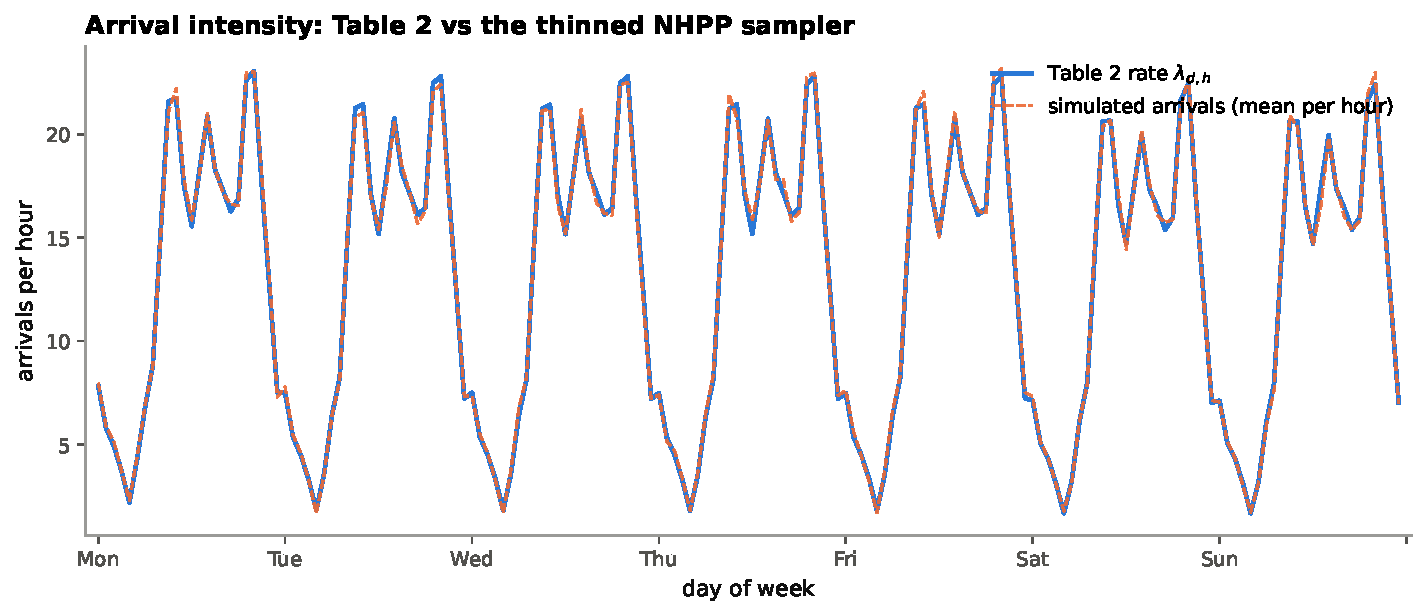
\includegraphics[width=\columnwidth]{figures/wp1_arrival_validation.pdf}
\caption{Validation of the thinned non-homogeneous Poisson arrival process
         against the base paper's published hourly rates.}
\Description{Two overlapping curves of arrivals per hour across a week; the
simulated curve tracks the published rate curve almost exactly across all
168 hourly bins.}
\label{fig:arrivals}
\end{figure}

Table~\ref{tab:validate} compares every KPI the paper publishes. Our model
matches the paper's patterns more closely than its exact numbers. The results
that agree closely are both service levels under IFP ($100\%/100\%$), ALT's
Level III waiting time ($6.05$ vs.\ $6.82$ published), SBP's Level III waiting
time ($12.35$ vs.\ $10.48$), physician utilisation ($86.3\%$ vs.\
$85.0$--$85.4\%$) and the fact that it barely changes across policies, and the
equipment-utilisation table (Table~\ref{tab:equip}), where all four modalities
are within $0.5$ percentage points. This supports the paper's main managerial
conclusion that physicians, not equipment, are the bottleneck.

\begin{table}[t]
\caption{Validation against the base paper. Deviation is relative to the
         published value; $100$ replications.}
\label{tab:validate}
\small
\begin{tabular}{@{}llrrr@{}}
\toprule
\textbf{Policy} & \textbf{Metric} & \textbf{Ours} & \textbf{Paper} & \textbf{Dev.} \\
\midrule
\multirow{4}{*}{IFP}
 & Mean wait, all (min)   & 52.43  & 46.26  & $+13.3\%$ \\
 & Mean wait, Level III   & 50.88  & 44.14  & $+15.3\%$ \\
 & Service level L3 / L4  & 100 / 100 & 100 / 100 & $0.0\%$ \\
 & Physician utilisation  & 86.36  & 85.43  & $+1.1\%$ \\
\midrule
\multirow{4}{*}{ALT}
 & Mean wait, all (min)   & 42.39  & 37.88  & $+11.9\%$ \\
 & Mean wait, Level III   & 6.05   & 6.82   & $-11.2\%$ \\
 & Service level L3 / L4  & 99.96 / 87.37 & 98.08 / 89.29 & $-2.2\%$ \\
 & Physician utilisation  & 86.34  & 85.41  & $+1.1\%$ \\
\midrule
\multirow{4}{*}{SBP}
 & Mean wait, all (min)   & 44.08  & 35.25  & $+25.1\%$ \\
 & Mean wait, Level III   & 12.35  & 10.48  & $+17.9\%$ \\
 & Service level L3 / L4  & 99.99 / 89.40 & 100 / 100 & $-10.6\%$ \\
 & Physician utilisation  & 86.34  & 84.98  & $+1.6\%$ \\
\bottomrule
\end{tabular}
\end{table}

\begin{table}[t]
\caption{Diagnostic equipment utilisation, reproduced from the base paper's
         Table 9.}
\label{tab:equip}
\small
\begin{tabular}{@{}lrrr@{}}
\toprule
\textbf{Equipment} & \textbf{Exams/week} & \textbf{Ours} & \textbf{Paper} \\
\midrule
Laboratory   & 1248 & 14.73\% & 14.36\% \\
X-ray        &  394 & 15.59\% & 15.20\% \\
CT           &  748 & 18.18\% & 17.64\% \\
B-ultrasound &  297 & 19.41\% & 19.03\% \\
\bottomrule
\end{tabular}
\end{table}

The absolute waiting times do not match: ours are $12$--$25\%$ higher. We
think this comes down to load. The published parameters imply
$\rho\approx0.870$, and close to saturation the mean wait is very sensitive to
small changes in utilisation. A small difference in the patient mix, which we
cannot recover, can therefore cause a large difference in waiting time. Since
the original dataset is not public, an exact numerical match is not possible
and we do not claim one. We report the gap as it is rather than adjusting
parameters to hit the published numbers.

\subsection{Policy comparison}
Table~\ref{tab:master} brings together all six policies, and
Figure~\ref{fig:tradeoff} shows the same results graphically. WSEPT has the
lowest holding cost ($0.3763$ compared with $0.7550$ for IFP, a $50\%$
reduction), as the Cox--Smith result predicts. On this system it also has the
lowest unweighted mean wait ($42.32$~min). All of its differences from the
paper's three heuristics remain significant after Bonferroni correction
(Table~\ref{tab:cmusig}).

\begin{table*}[t]
\caption{Comparison of all six scheduling policies; $100$ common-random-number
         replications. SBP$^{*}$ is the Slack-Based Policy with our constrained
         Nelder--Mead thresholds. ``Meets SLA'' requires $SL_\ell\ge95\%$ on
         \emph{both} triage levels.}
\label{tab:master}
\begin{tabular}{@{}llrlrrrrrrc@{}}
\toprule
\textbf{Policy} & \textbf{Origin} & \textbf{Wait (min)} & \textbf{95\% CI} &
\textbf{L-III} & \textbf{L-IV} & \textbf{Holding} &
\textbf{$SL_3$} & \textbf{$SL_4$} & \textbf{Util.} & \textbf{Meets SLA} \\
\midrule
IFP    & base paper                & 52.43 & [49.63, 55.22] & 50.88 & 52.94 & 0.7550 & 100.00\% & 100.00\% & 86.36\% & yes \\
ALT    & base paper                & 42.39 & [40.26, 44.51] & 6.05  & 54.61 & 0.3913 & 99.96\%  & 87.37\%  & 86.34\% & \textbf{no} \\
SBP    & base paper $(13.1,2.1)$   & 44.08 & [41.72, 46.44] & 12.35 & 54.74 & 0.4450 & 99.99\%  & 89.40\%  & 86.34\% & \textbf{no} \\
SBP$^{*}$ & \textbf{ours} $(2.31,8.37)$ & 44.18 & [41.81, 46.55] & 14.14 & 54.27 & 0.4570 & 95.42\%  & 95.64\%  & 86.34\% & \best{yes} \\
WSEPT  & \textbf{ours}, c$\mu$     & \best{42.32} & [40.21, 44.43] & 3.76 & 55.30 & \best{0.3763} & 100.00\% & 86.87\% & 86.34\% & \textbf{no} \\
Gc$\mu$& \textbf{ours}, gen.\ c$\mu$ & 44.05 & [41.81, 46.29] & 14.59 & 53.94 & 0.4588 & 100.00\% & 90.99\%  & 86.35\% & \textbf{no} \\
\bottomrule
\end{tabular}
\end{table*}

\begin{table}[t]
\caption{Paired $t$-tests on the holding cost, WSEPT against every other
         policy. Bonferroni-adjusted $\alpha = 0.00333$.}
\label{tab:cmusig}
\small
\begin{tabular}{@{}lrrrr@{}}
\toprule
\textbf{Comparison} & \textbf{Diff.} & $t$ & $p$ & \textbf{Cohen's $d$} \\
\midrule
IFP vs.\ WSEPT    & $+0.3786$ & 31.67  & $1.3\!\times\!10^{-53}$ & 3.17 \\
ALT vs.\ WSEPT    & $+0.0150$ & 36.54  & $2.9\!\times\!10^{-59}$ & 3.65 \\
SBP vs.\ WSEPT    & $+0.0686$ & 14.15  & $1.6\!\times\!10^{-25}$ & 1.42 \\
WSEPT vs.\ Gc$\mu$& $-0.0824$ & $-33.42$ & $1.0\!\times\!10^{-55}$ & $-3.34$ \\
\bottomrule
\end{tabular}
\end{table}

\begin{figure}[t]
\centering
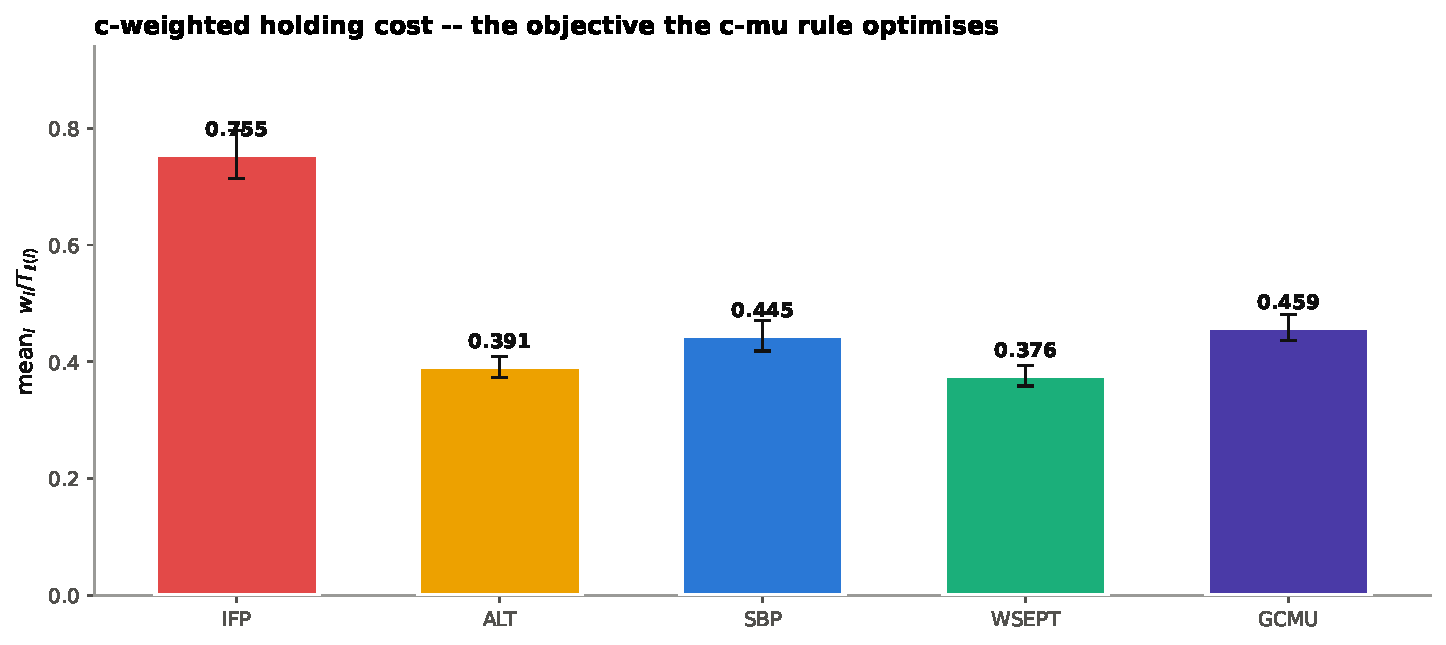
\includegraphics[width=\columnwidth]{figures/wp2_holding_cost_bars.pdf}
\caption{Holding cost by policy, the objective the c$\mu$ rule is optimal for.
         Each patient's wait is measured relative to their own clinical target
         (Eq.~\eqref{eq:holding}). Lower is better.}
\Description{Bar chart of holding cost by policy. IFP is about 0.755, roughly
twice every other policy; WSEPT is lowest at 0.376, followed by ALT, SBP and
generalised c-mu.}
\label{fig:holding}
\end{figure}

The service-level columns of Table~\ref{tab:master} show the main trade-off:
the policies that serve Level III patients fastest are the same ones that let
Level IV patients miss their target. WSEPT reaches only $86.9\%$ on Level IV,
ALT is similar, and the paper's own tuned SBP reaches $89.4\%$. Only IFP, which
is slow, and our re-tuned SBP$^{*}$ meet the constraint on both levels. So
there is no single best policy, and the answer depends on the objective. WSEPT
gives the lowest holding cost and the lowest raw mean wait, while SBP$^{*}$ is
the fastest policy a hospital could adopt under the $95\%$ constraint.

\begin{figure}[t]
\centering
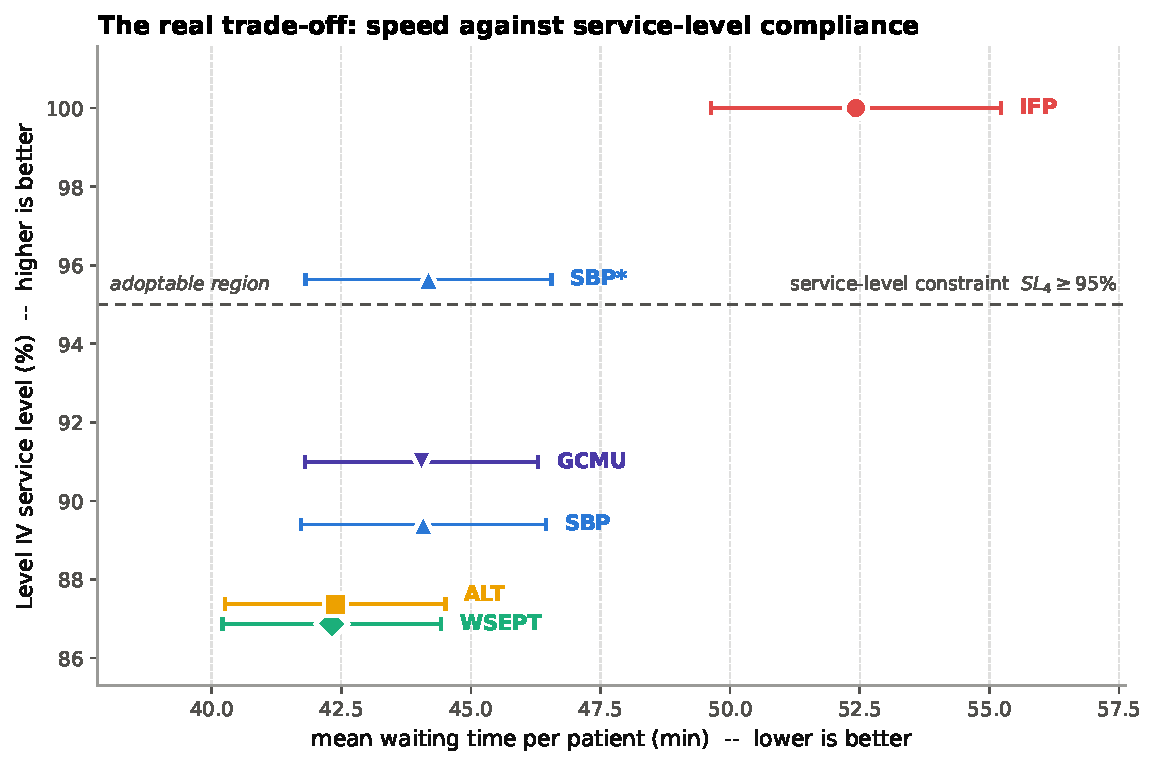
\includegraphics[width=\columnwidth]{figures/final_tradeoff.pdf}
\caption{Speed against service-level compliance. Only policies above the dashed
         constraint line can be adopted. Among the tuned policies, only
         SBP$^{*}$ is both fast and feasible.}
\Description{Scatter plot with mean waiting time on the horizontal axis and
Level IV service level on the vertical axis. IFP sits top right, slow but at
100 percent. ALT, WSEPT, SBP and generalised c-mu sit bottom left, fast but
below the 95 percent dashed line. SBP star sits just above the line at about
44 minutes.}
\label{fig:tradeoff}
\end{figure}

There is one caveat. The Cox--Smith optimality proof assumes a single-stage
multi-class queue. Our model has re-entrant flow, since patients come back for
a follow-up after diagnostics, and the number of physicians changes over time.
The optimality guarantee therefore holds only approximately here, so we rely
on the observed ranking rather than on the theorem.

\subsection{Optimiser versus brute force}
\label{sec:resopt}
Table~\ref{tab:budget} shows the main efficiency result. When we ran the
paper's procedure on our model, the two-stage grid evaluated $2{,}332$ points.
That took $50{,}415$ week-long simulations, roughly $970$ simulated
patient-years of ED operation, and ended at $(4.10,8.20)$. Our simplex found an
equally good point with $2{,}650$ simulations, which is $19.0$ times fewer.
When both optima were re-evaluated on the same full-length batch, they
differed by $0.006$ minutes, well below the noise of the simulation.

\begin{table}[t]
\caption{Simulation budget required by brute-force grid search and by our
         Nelder--Mead simplex, on the same objective and the same patient
         streams.}
\label{tab:budget}
\small
\begin{tabular}{@{}lrrr@{}}
\toprule
\textbf{Method} & \textbf{Points} & \textbf{Simulations} & \textbf{Objective} \\
\midrule
Grid, coarse (step 1.0)  & 1{,}891 & 28{,}365 & 47.6105 \\
Grid, fine (step 0.1)    &    441  & 22{,}050 & 46.4601 \\
\textbf{Grid, total}     & 2{,}332 & \textbf{50{,}415} & 46.4601 \\
Nelder--Mead, 1 start    &     53  & \best{2{,}650} & 46.4668 \\
Nelder--Mead, 4 starts   &    196  & 9{,}800  & 46.4668 \\
\bottomrule
\end{tabular}
\end{table}

Starting from four different points, the runs ended with objective values
within $0.15$~min of each other ($46.468$--$46.622$). This suggests that the
penalised surface has a single minimum inside this box. Our implementation also
agrees with \texttt{scipy.optimize} to $0.0000$~min on the same objective.
Figure~\ref{fig:path} shows the simplex path over the response surface that the
grid had to evaluate point by point, and Figure~\ref{fig:conv} plots solution
quality against budget.

\begin{figure}[t]
\centering
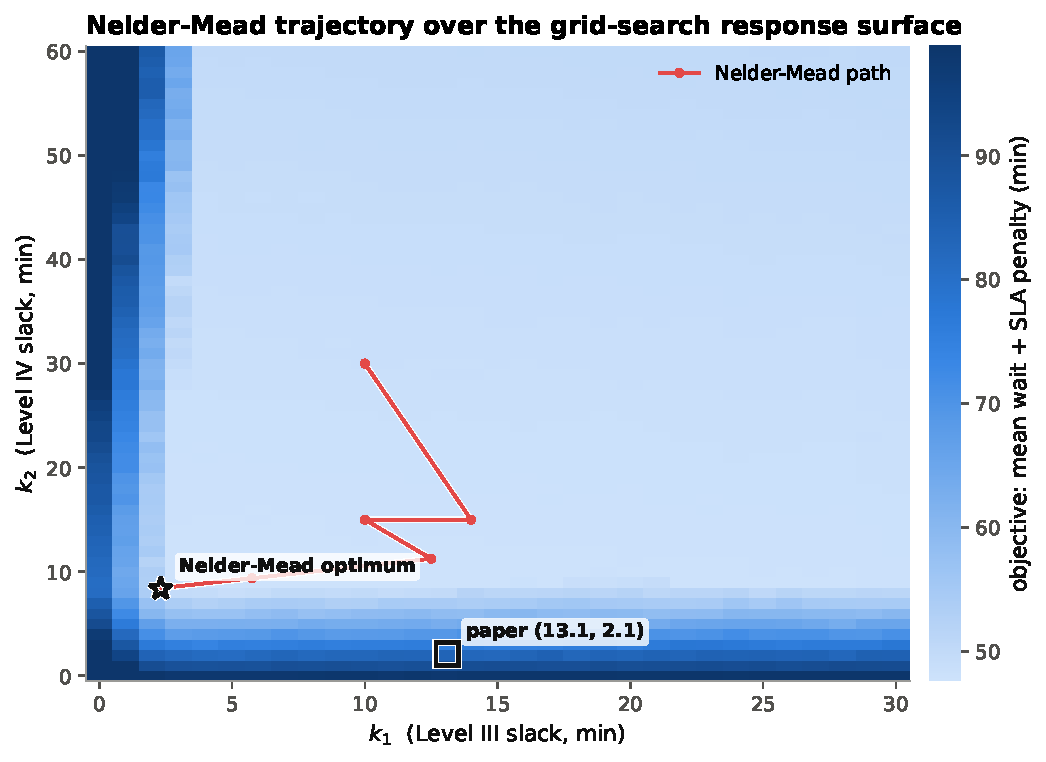
\includegraphics[width=\columnwidth]{figures/wp3_simplex_path.pdf}
\caption{The Nelder--Mead path over the grid-search response surface. The dark
         band is the service-level penalty region; the base paper's published
         optimum (square) lies inside it.}
\Description{Heat map over k1 and k2 with a dark high-penalty band along the
bottom edge. A red path descends from the start point at (10, 30) to a star
marking the converged optimum near (2.3, 8.4). A square marks the paper
optimum at (13.1, 2.1) inside the dark band.}
\label{fig:path}
\end{figure}

\begin{figure}[t]
\centering
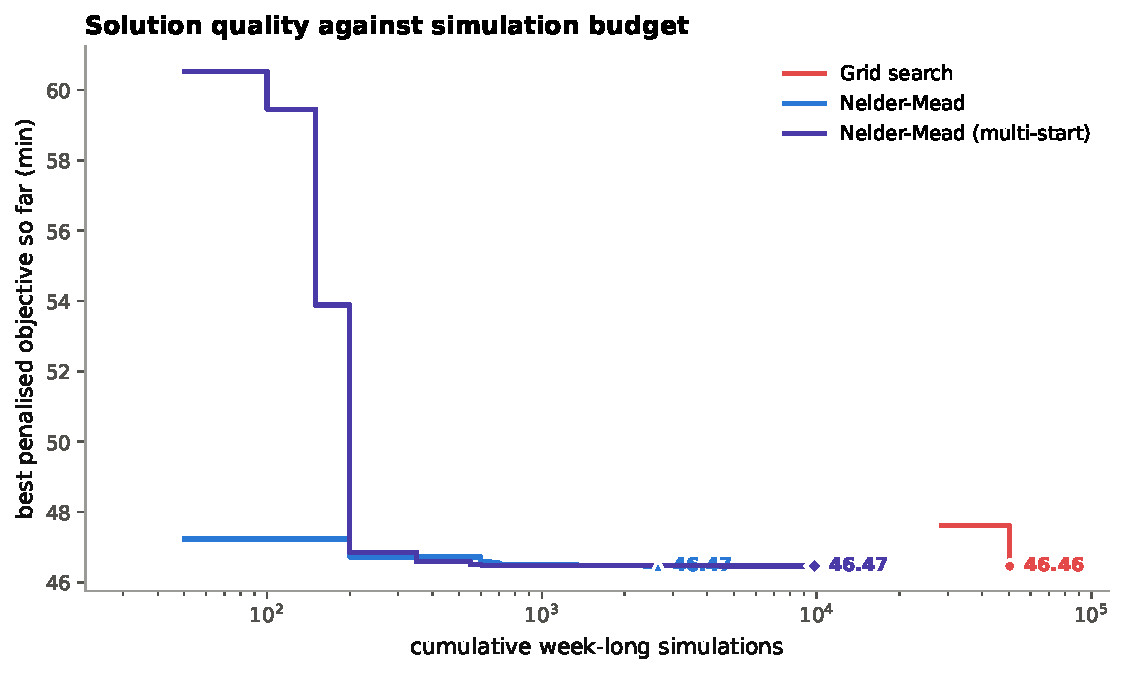
\includegraphics[width=\columnwidth]{figures/wp3_convergence.pdf}
\caption{Best objective found so far against cumulative simulation budget
         (log scale).}
\Description{Step plot of best objective versus number of simulations on a
logarithmic horizontal axis. The Nelder-Mead curves reach the same objective
level as grid search at roughly one twentieth of the budget.}
\label{fig:conv}
\end{figure}

This experiment also gave a result we did not expect. With the $95\%$
constraint in place, the optimum shifts to a much larger $k_2$, and the
paper's published $(13.1,2.1)$ becomes \emph{infeasible} on our model, reaching
only $89.4\%$ on Level IV (Table~\ref{tab:optconf}). The reason is simple. With
$T_4=120$ and $k_2=2.1$, a Level IV patient is flagged urgent only after
waiting $117.9$ of their $120$ allowed minutes, which leaves too little time to
see them in a system this congested. This is the clearest case in our work for
re-tuning under an explicit constraint instead of reusing published
parameters.

\begin{table}[t]
\caption{All three optima re-evaluated on the same replications.}
\label{tab:optconf}
\small
\begin{tabular}{@{}llrrrl@{}}
\toprule
\textbf{Setting} & $(k_1,k_2)$ & \textbf{Wait} & $SL_3$ & $SL_4$ & \textbf{Status} \\
\midrule
Nelder--Mead    & $(2.31, 8.37)$ & 44.18 & 95.42\% & 95.64\% & feasible \\
Grid search     & $(4.10, 8.20)$ & 44.17 & 97.73\% & 95.49\% & feasible \\
Paper           & $(13.10, 2.10)$& 44.08 & 99.99\% & 89.40\% & \textbf{infeasible} \\
\bottomrule
\end{tabular}
\end{table}

\subsection{Cost-optimal staffing}
\label{sec:resstaff}
Table~\ref{tab:staffing} prices the paper's seven staffing scenarios using
Eq.~\eqref{eq:cost}. On its own, the paper can only say that more physicians
give shorter waits, which does not tell a hospital where to stop. Once the
scenarios are priced, the cost is lowest at $S_5$. A free search over all $140$
admissible rosters, with $(k_1,k_2)$ re-tuned inside each one, finds a cheaper
option: roster $(6,6,3)$ with thresholds $(12.20, 23.40)$. Compared with the
paper's fixed $(5,5,3)$, it uses $105$ more physician-hours per week, but it
cuts mean waiting by $33$ minutes per patient and reduces the SLA penalty from
$4{,}913$ to $60$ cost units. The net weekly saving is $28{,}878$ units, or
$20.7\%$.

\begin{table}[t]
\caption{The base paper's seven staffing scenarios, priced using
         Eq.~\eqref{eq:cost}. Cost in arbitrary units per week.}
\label{tab:staffing}
\small
\begin{tabular}{@{}llrrrr@{}}
\toprule
& \textbf{Roster} & \textbf{Phys-h} & \textbf{Wait} & $SL_4$ & \textbf{Total} \\
\midrule
$S_0$ & (5,5,3) & 714  & 44.18 & 95.64\%  & 139{,}391 \\
$S_1$ & (5,5,4) & 777  & 35.19 & 98.53\%  & 134{,}121 \\
$S_2$ & (5,5,5) & 840  & 31.25 & 99.32\%  & 136{,}490 \\
$S_3$ & (5,6,5) & 889  & 16.34 & 99.98\%  & 124{,}942 \\
$S_4$ & (5,7,5) & 938  & 11.45 & 100.00\% & 125{,}327 \\
$S_5$ & (6,7,5) & 994  & 4.32  & 100.00\% & \best{124{,}082} \\
$S_6$ & (7,7,5) & 1050 & 2.38  & 100.00\% & 128{,}652 \\
\midrule
\multicolumn{2}{@{}l}{\textbf{Ours} (6,6,3)} & 819 & 10.97 & 99.93\% & \best{110{,}513} \\
\bottomrule
\end{tabular}
\end{table}

Optimising roster and thresholds together makes a measurable difference.
Roster $(6,6,3)$ scores $111{,}932$ when screened at one fixed threshold pair
and $110{,}870$ after re-tuning to its own optimum $(12.20,23.40)$. More
importantly, the best thresholds change a lot from one roster to another, with
$k_2$ ranging from $11.5$ to $25.6$ across the six refined candidates. Keeping
them fixed while varying staffing would mean scoring each roster with
thresholds chosen for a different one.

\begin{table}[t]
\caption{Sensitivity of the staffing recommendation to the cost weights.}
\label{tab:costsens}
\small
\begin{tabular}{@{}lrrrlr@{}}
\toprule
\textbf{Scenario} & $\alpha$ & $\beta$ & $\gamma$ & \textbf{Winner} & \textbf{vs.\ (5,5,3)} \\
\midrule
Baseline              & 120 & 0.500 & 50  & (6,6,3) & $-20.7\%$ \\
Waiting $\times4$     & 120 & 2.000 & 50  & (6,7,3) & $-53.2\%$ \\
Waiting $\times\!\frac{1}{4}$ & 120 & 0.125 & 50 & (5,6,3) & $-5.2\%$ \\
Physicians $\times1.5$& 180 & 0.500 & 50  & (6,6,3) & $-12.4\%$ \\
SLA breach $\times10$ & 120 & 0.500 & 500 & (6,6,3) & $-39.5\%$ \\
\bottomrule
\end{tabular}
\end{table}

Table~\ref{tab:costsens} tests how sensitive the recommendation is to the cost
weights. The best roster does change with the weights. We see this as a result
in itself rather than a weakness of the method: the right staffing level
depends on how a hospital values a minute of patient waiting against a
physician's salary, so those weights have to be agreed on before a roster is
chosen. In every weighting we tried, though, the best roster is cheaper than
the paper's fixed $(5,5,3)$, by between $5.2\%$ and $53.2\%$.

\begin{figure}[t]
\centering
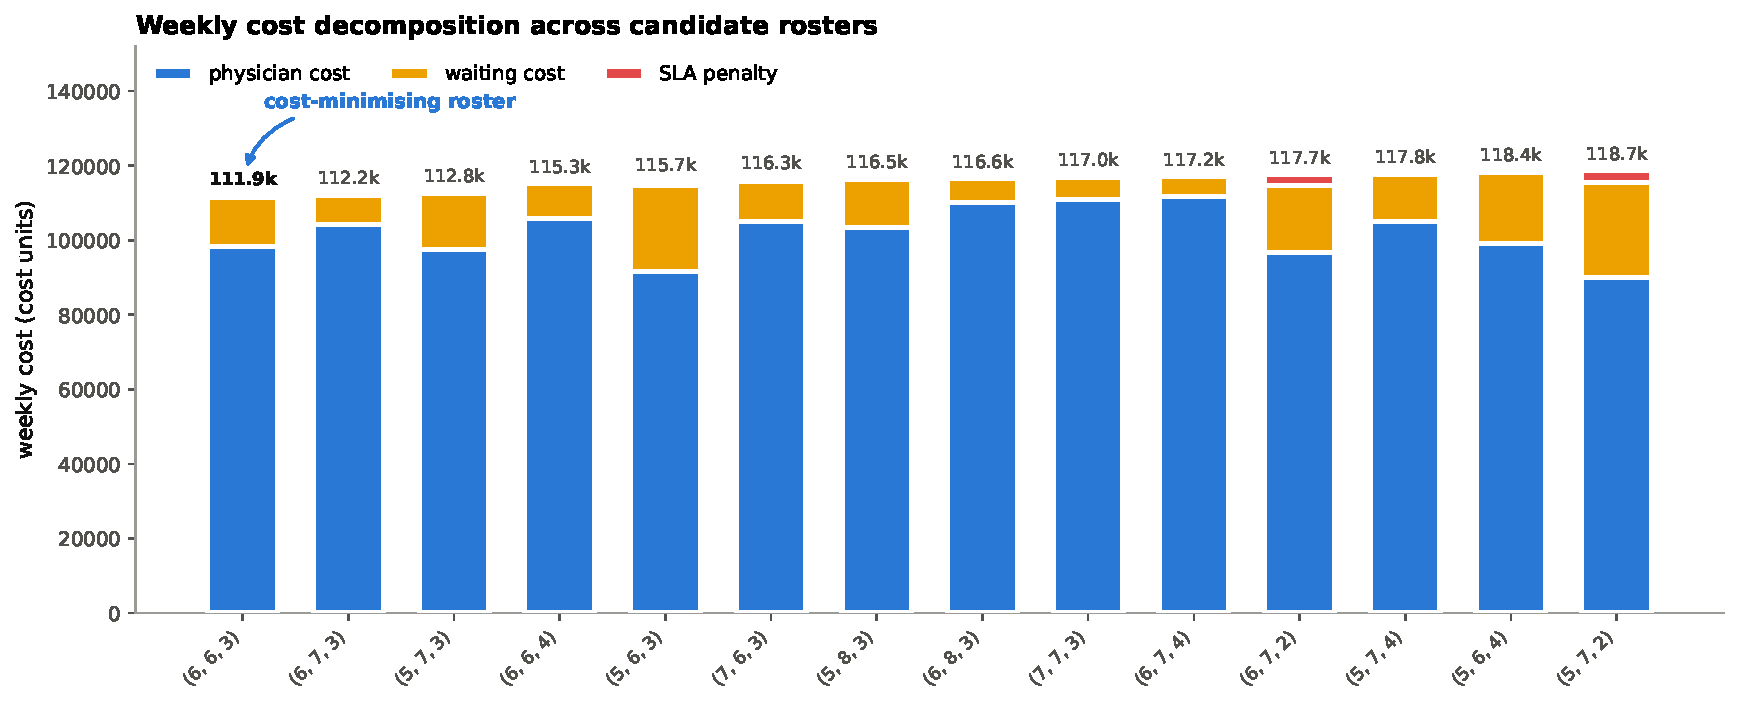
\includegraphics[width=\columnwidth]{figures/wp4_cost_decomposition.pdf}
\caption{Weekly cost split into physician, waiting and SLA-penalty components
         for the best screened rosters.}
\Description{Stacked bar chart across fourteen candidate rosters. Physician
cost dominates each bar; waiting cost shrinks as staffing rises while physician
cost grows, producing a minimum total at roster six six three.}
\label{fig:cost}
\end{figure}

\subsection{Variance reduction}
Table~\ref{tab:crn} shows the effect of CRN on every pairwise comparison. The
correlations between paired results range from $+0.996$ to $+0.9996$, compared
with about $0$ for independent streams. The median reduction in variance is
$98.95\%$, which corresponds to a median efficiency gain of $95.8\times$.
Confidence intervals on the mean differences become $4$ to $40$ times
narrower.

\begin{table}[t]
\caption{Variance of the pairwise difference in mean waiting time, with and
         without common random numbers; $100$ replications per arm.}
\label{tab:crn}
\small
\begin{tabular}{@{}lrrrr@{}}
\toprule
\textbf{Comparison} & \textbf{Var ind.} & \textbf{Var CRN} & \textbf{Removed} & \textbf{Gain} \\
\midrule
IFP vs.\ ALT     & 241.34 & 12.44 & 94.85\% & 19.4$\times$ \\
IFP vs.\ SBP     & 330.48 & 6.12  & 98.15\% & 54.0$\times$ \\
IFP vs.\ WSEPT   & 288.20 & 13.16 & 95.43\% & 21.9$\times$ \\
IFP vs.\ Gc$\mu$ & 216.19 & 8.50  & 96.07\% & 25.4$\times$ \\
ALT vs.\ SBP     & 220.77 & 2.15  & 99.03\% & 102.9$\times$ \\
ALT vs.\ WSEPT   & 191.64 & 0.11  & 99.94\% & 1789.3$\times$ \\
ALT vs.\ Gc$\mu$ & 223.75 & 0.46  & 99.79\% & 485.4$\times$ \\
SBP vs.\ WSEPT   & 198.04 & 2.23  & 98.87\% & 88.7$\times$ \\
SBP vs.\ Gc$\mu$ & 268.97 & 1.03  & 99.62\% & 261.8$\times$ \\
WSEPT vs.\ Gc$\mu$& 215.27 & 0.59 & 99.72\% & 362.7$\times$ \\
\midrule
\multicolumn{3}{@{}l}{\textbf{Median}} & \best{98.95\%} & \best{95.8$\times$} \\
\bottomrule
\end{tabular}
\end{table}

Two points are worth noting. First, CRN does not bias the results. The
per-policy means and standard deviations agree between the two arms within
sampling error, as expected, since CRN only changes the joint distribution.
Second, it can change conclusions. Several comparisons that do not pass the
Bonferroni threshold with independent streams become clearly significant under
CRN. Where the two arms disagree, the CRN result is the more reliable one,
because it estimates the same quantity with lower variance.

A $95.8\times$ efficiency gain does not mean that one replication is enough.
The ratio is itself an estimate, and a $t$-interval needs enough degrees of
freedom. A safer practical reading is that $20$--$30$ CRN replications give
comparisons at least as precise as the base paper's $100$ independent ones,
which is still a $3$--$5\times$ saving.

\begin{figure}[t]
\centering
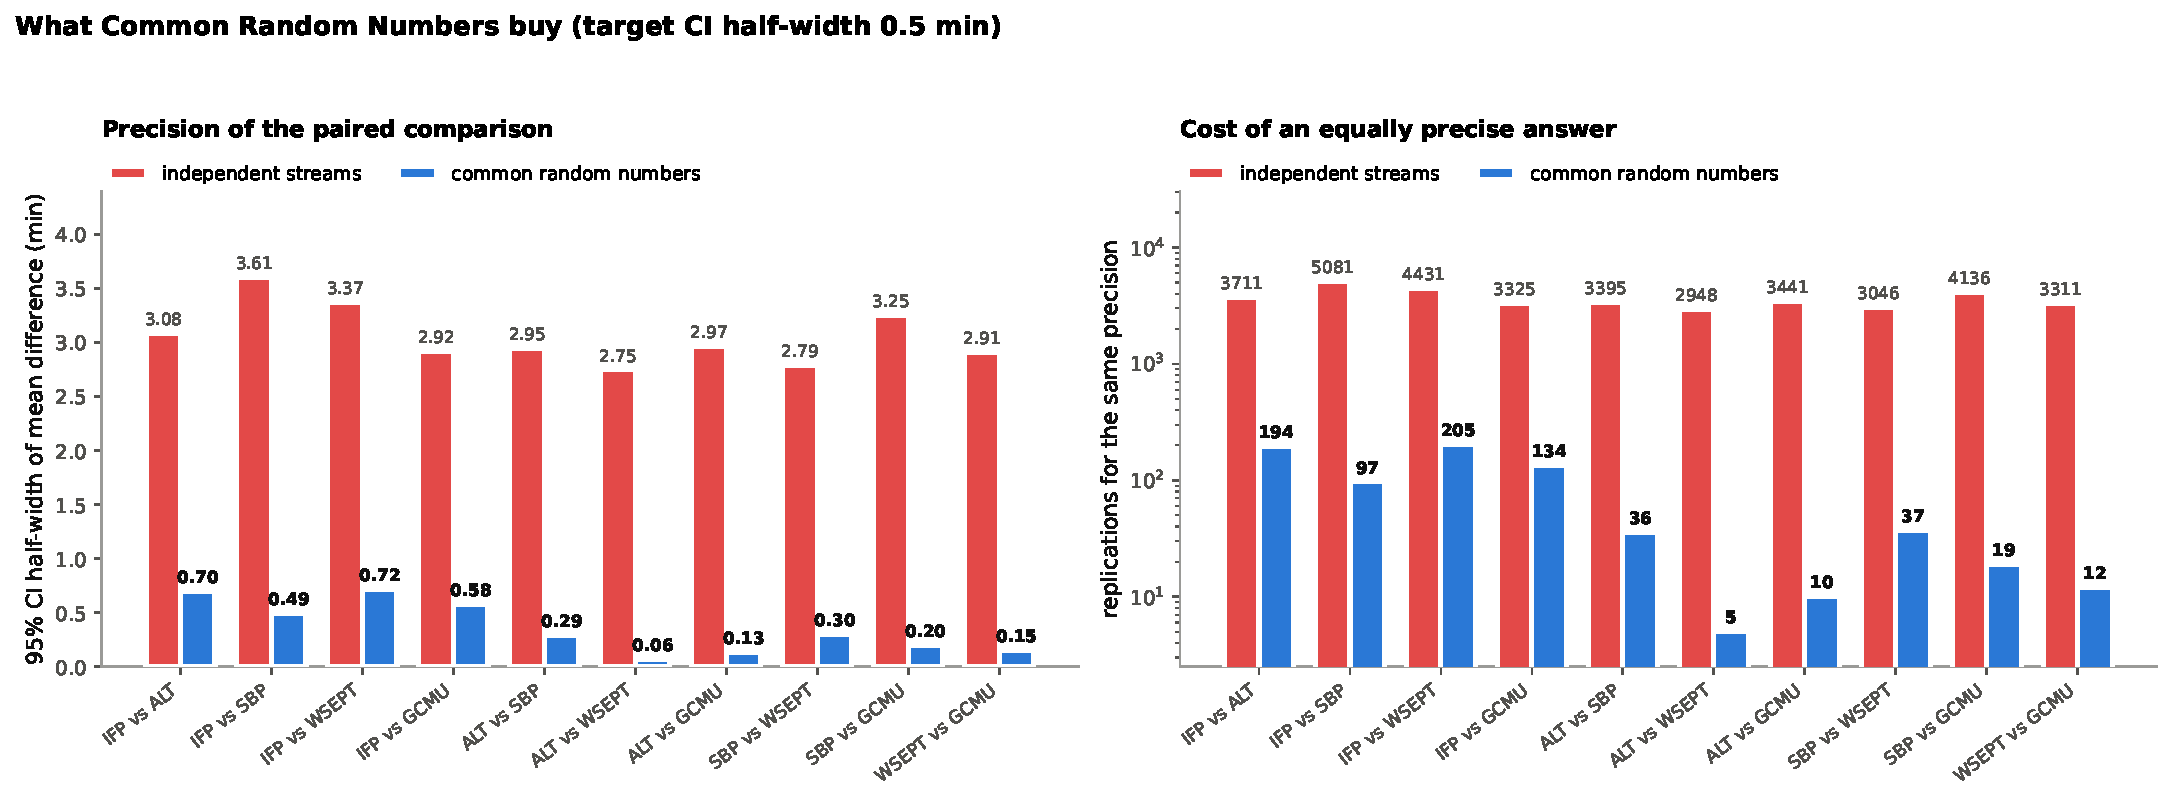
\includegraphics[width=\columnwidth]{figures/wp5_crn_variance_reduction.pdf}
\caption{Left: 95\% confidence-interval half-width on each pairwise difference.
         Right: replications needed for $\pm0.5$~min precision (log scale).}
\Description{Two grouped bar charts over ten policy pairs. In both, the common
random numbers bars are far shorter than the independent stream bars; the
right panel shows thousands of replications reduced to tens.}
\label{fig:crn}
\end{figure}

\subsection{Robustness}
We repeat all three of the base paper's sensitivity studies and include the
added policies. Scaling all arrival rates from $-15\%$ to $+15\%$
(Figure~\ref{fig:arr}) moves $\rho$ from $0.739$ to $1.000$. Under light load
the policies perform almost the same, and they separate sharply as the system
approaches saturation, with the gap between them growing from $1.6$ to
$53$~min. Across the seven staffing scenarios (Figure~\ref{fig:staff}), waits
fall with diminishing returns, and the choice of policy matters most when
physicians are scarce: the gap shrinks from $10.1$~min at $S_0$ to $0.06$~min
at $S_6$. Finally, replacing the truncated exponential service times with
truncated lognormals that have the same nominal means raises all waits by
$44$--$54\%$ because of the heavier right tail, but the ranking stays exactly
the same. The comparative conclusions therefore do not depend on the choice of
service-time distribution. All three findings agree with the base paper.

\begin{figure}[t]
\centering
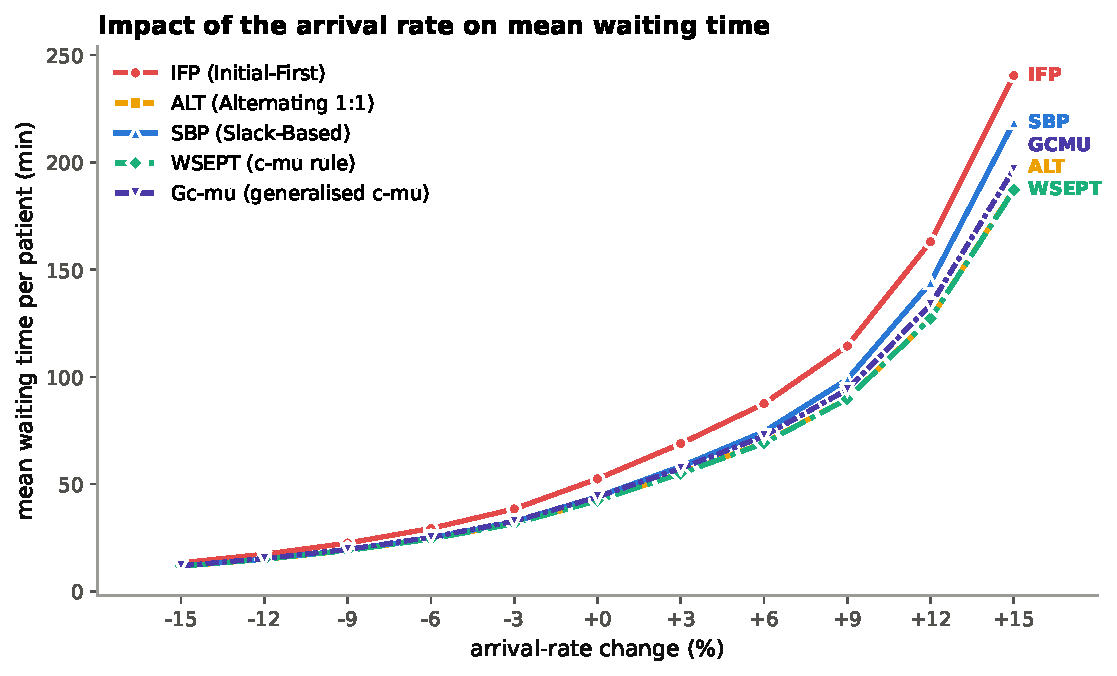
\includegraphics[width=\columnwidth]{figures/sens_arrival_rate.pdf}
\caption{Effect of the arrival rate on mean waiting time, all five policies.}
\Description{Five rising curves of mean waiting time against arrival rate
change from minus fifteen to plus fifteen percent. All curves coincide at the
left and fan out steeply at the right, with IFP highest throughout.}
\label{fig:arr}
\end{figure}

\begin{figure}[t]
\centering
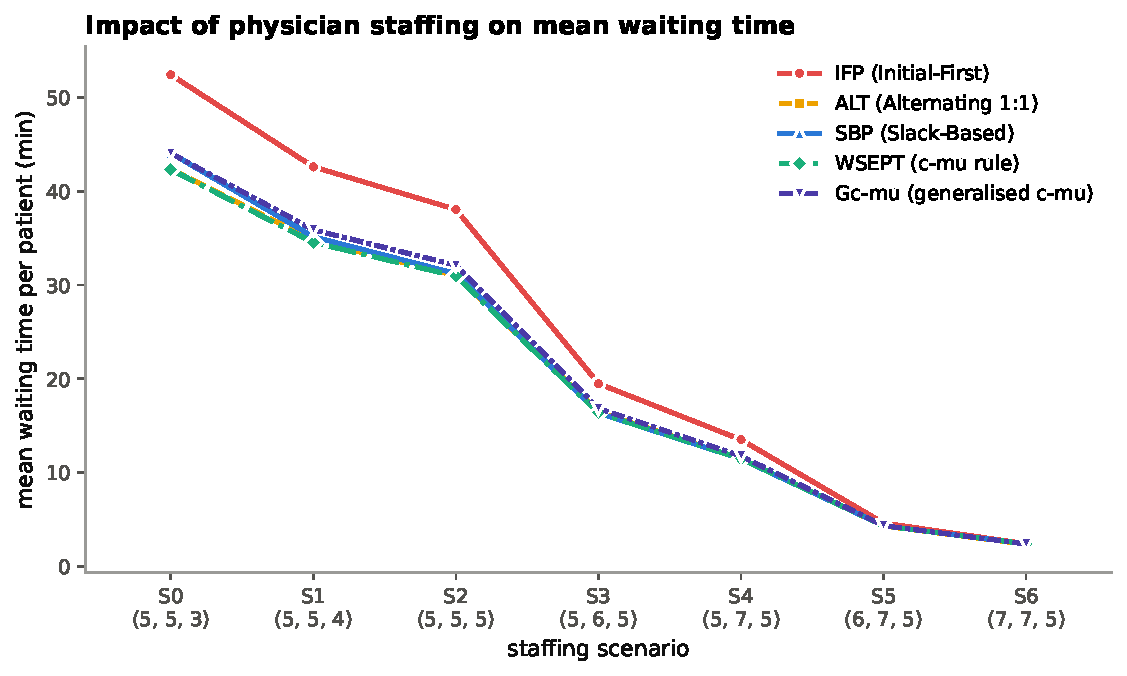
\includegraphics[width=\columnwidth]{figures/sens_staffing.pdf}
\caption{Effect of physician staffing on mean waiting time across the base
         paper's seven scenarios.}
\Description{Five descending curves of mean waiting time across staffing
scenarios S0 to S6. The curves are separated at S0 and converge to almost the
same value by S6.}
\label{fig:staff}
\end{figure}

\subsection{Threats to validity}
Our claims have three main limitations. \emph{Construct validity}: the base
paper's dataset is not available, so we calibrate only to published summary
statistics. The $12$--$25\%$ gap in waiting times is the visible result of
this, and only the relative conclusions should be relied on. \emph{Internal
validity}: five parameters were chosen by us. Four of them are varied or
stress-tested, and for the fifth ($SL^{\min}$) we report both raw service
levels so that readers can apply a different threshold themselves.
\emph{External validity}: the model covers one ED with one triage system, the
c$\mu$ optimality guarantee is weakened by re-entrant flow, and the cost
weights are illustrative rather than taken from a real hospital.

%% ======================================================================
\section{Conclusion and Future Work}

We rebuilt the discrete-event model of Lv et al.~\cite{lv2026des} using only
its published parameters and compared it with every KPI the paper reports. All
six structural findings carry over, including the equipment-utilisation table
(within $0.5$ percentage points) and the conclusions of all three sensitivity
analyses. Absolute waiting times are $12$--$25\%$ higher, which we attribute to
the high implied load $\rho\approx0.87$. We report this gap instead of tuning
it away.

We then added four extensions. A policy based on the c$\mu$ rule, which is
optimal for a stated delay-cost objective, gives the lowest holding cost
($50\%$ below IFP) and the lowest raw mean wait. Our Nelder--Mead
implementation with an exterior penalty comes within $0.006$~min of the
grid-search optimum while using $19\times$ fewer week-long simulations. An
explicit cost model shows that roster $(6,6,3)$ with re-tuned thresholds is
$20.7\%$ cheaper per week than the paper's fixed $(5,5,3)$, although the best
roster depends on the cost weights, which we report as a finding. Exact common
random numbers remove $98.9\%$ of the variance in every pairwise comparison.

Our most important result is a negative one. On our model, the paper's
published thresholds $(13.1, 2.1)$ break a $95\%$ Level IV service-level
constraint, because $k_2 = 2.1$ delays intervention until minute $117.9$ of
$120$. Re-tuning under the constraint fixes this and gives the only tuned
policy a hospital could adopt. Scheduling parameters fitted to one system
should not be assumed to carry over to another.

We see three directions for future work. The c$\mu$ guarantee could be
re-derived for the re-entrant, time-varying setting studied here, for which
only asymptotic results currently exist. The optimiser could be applied to
larger decision vectors, such as per-shift thresholds or thresholds that depend
on the current queue state. There the advantage over grid search grows
quickly, and the base paper itself suggests reinforcement learning for this.
Finally, the cost model could be set up as a stochastic program, with the
roster as a first-stage decision and the thresholds as a recourse decision.
This would replace our two-stage screening heuristic with a proper
decomposition.

%% ======================================================================
\begin{acks}
We thank the course instructors of CSE~402 for their guidance on scope and
methodology. All simulation code, generated result tables, figures and a
provenance log recording the exact command behind every output are available
at \url{\REPOURL}.
\end{acks}

\bibliographystyle{ACM-Reference-Format}
\bibliography{references}

\end{document}